%%%%%%%%%%%%%%%%%%%%%%%%%%%%%%%%%%%%%%%%%%%%%%%%%%%%%%%%%%%%%%%%%%%%%%%%%%%%%%%%
\documentclass[conference]{IEEEtran}

\usepackage[utf8]{inputenc}
\usepackage[T1]{fontenc}
\usepackage{graphicx}
\usepackage{booktabs}
\usepackage{amsmath}
\usepackage{hyperref}
\usepackage{subcaption}
\usepackage{multirow}

% tighten float spacing
\setlength{\textfloatsep}{4pt plus 1pt minus 1pt}
\setlength{\floatsep}{3pt plus 1pt minus 1pt}
\setlength{\intextsep}{3pt plus 1pt minus 1pt}
\setlength{\abovecaptionskip}{3pt}
\setlength{\belowcaptionskip}{2pt}

\title{\LARGE \bf
Reinforcement Learning Report: \\
Matching Algorithms to MDP Structure on Blackjack and CartPole
}

\author{
\parbox{3in}{
\centering
Michael Ciniello \\
School of Computer Science \\
Georgia Institute of Technology \\
Atlanta, GA, USA \\
{\tt\small mciniello3@gatech.edu}
}
}

\begin{document}

\maketitle
\thispagestyle{empty}
\pagestyle{empty}


%%%%%%%%%%%%%%%%%%%%%%%%%%%%%%%%%%%%%%%%%%%%%%%%%%%%%%%%%%%%%%%%%%%%%%%%%%%%%%%%
\section{Introduction and Environments}

This report studies how the structural properties of a Markov Decision
Process (MDP) --- discrete vs.\ continuous state, stochastic vs.\ (nearly)
deterministic dynamics --- interact with the algorithm family chosen to
solve it. We use two environments that sit at opposite ends of both axes:

\textbf{Blackjack}~\cite{sutton2018} is inherently discrete and stochastic.
State is a tuple $(\text{player sum}, \text{dealer card}, \text{usable ace})$
with 360 non-terminal states. Actions are
$\{\text{hit}, \text{stick}\}$. Reward is terminal: $+1$ for winning, $-1$
for losing, $0$ for drawing, and is delivered only at episode end.
Gymnasium's \texttt{Blackjack-v1}~\cite{gym_blackjack} only exposes
\texttt{step}/\texttt{reset} --- it does not expose $T$ or $R$ --- so
running VI/PI requires an explicit model. We build the analytical MDP
from scratch, enumerating hit and stick transitions state-by-state from
the rules of the game. This gives VI and PI access to the
\emph{exact} Bellman optimum rather than an estimate, and is what makes
Blackjack load-bearing in our study: it is the one environment where the
model-free gap to $V^*$ can be measured rather than inferred.

\textbf{CartPole-v1}~\cite{barto1983, gym_cartpole} is continuous and
\emph{nearly} deterministic --- the dynamics themselves (Euler-integrated
equations of motion) are fully deterministic; stochasticity enters only at
\texttt{reset}, where each of the four state components is drawn uniformly
from $[-0.05, 0.05]$ (cart near track centre, pole nearly upright with a
tiny lean, essentially at rest). State is a 4-vector $(x, \dot{x}, \theta,
\dot\theta)$: cart position (m), cart velocity (m/s), pole angle (rad from
vertical), and pole angular velocity (rad/s). Actions are $\{\text{push
left}, \text{push right}\}$; reward is $+1$ per surviving timestep, capped
at 500. There is no natural tabular MDP --- any model requires
discretization. For the tabular model-free agents we follow the FAQ's
non-uniform binning guidance~\cite{cartpole_faq}, clamping $(x, \dot{x},
\theta, \dot\theta)$ to $[-2.4, 2.4] \times [-3, 3] \times [-0.2, 0.2]
\times [-3.5, 3.5]$ and using grid $(3, 3, 8, 12) = 864$ non-terminal cells
as the default, ablating across $(1,1,6,6)$ through $(5,5,12,16)$.
Running VI/PI on CartPole likewise requires an explicit model, but unlike
Blackjack we have no closed-form transitions to enumerate. Instead, we
roll out a sampling policy, count transitions per $(s_{\text{bin}}, a,
s'_{\text{bin}})$, and normalize to build an empirical $(T, R)$ that
VI/PI consume. The quality of the resulting DP policy then depends heavily
on the choice of sampling policy --- a point we return to in
Hypothesis~2 (Sec.~\ref{sec:hypotheses}).

\textbf{Reference optima.} For Blackjack, the exact Bellman fixed
point $V^*$ from VI/PI on the analytical MDP is our ground-truth
optimum --- we refer to it as the \emph{DP optimum} throughout.
CartPole has no closed-form $V^*$, so we use two reference points
instead: the 500-step truncation ceiling (practical best), and the
best DP policy at a matched grid (intrinsically grid- and
sampling-dependent, not a property of the environment).


%%%%%%%%%%%%%%%%%%%%%%%%%%%%%%%%%%%%%%%%%%%%%%%%%%%%%%%%%%%%%%%%%%%%%%%%%%%%%%%%
\section{Hypotheses}
\label{sec:hypotheses}

We organize the campaign around five predictions registered
ahead of data, structured along two axes: \emph{model
availability} (exact $\to$ DP dominates; estimated $\to$
sampling drives outcomes) and \emph{representation match}
(tabular suits discrete states, function approximation suits
continuous). The meta-prediction (H0) is that MDP structure,
not tuning, should decide which algorithm family wins.
H1--H5 operationalize this:

\begin{itemize}
\itemsep0em
\item \textbf{H1} (Blackjack DP): VI and PI reach the same $V^*$
on the analytical MDP; VI uses fewer Bellman backups than PI at
$\gamma = 1$ (weak contraction forces PI's inner PE loop to run
more sweeps per outer round).
\item \textbf{H2} (CartPole DP sampling): DP quality on the
estimated MDP is highly sensitive to sampling policy;
trained-$\varepsilon$ beats random, especially on fine grids
where random rollouts under-cover $(s, a)$ space.
\item \textbf{H3} (SARSA $\approx$ Q-L): Neither MDP has
cliff-walking geometry, so SARSA and Q-Learning match within
seed noise on both environments.
\item \textbf{H4} (CartPole discretization + $\gamma$):
Pole-axis resolution dominates cart-axis; CartPole is
$\gamma$-sensitive (long horizon), Blackjack is not (terminal
rewards).
\item \textbf{H5} (DQN + Rainbow, EC): Vanilla DQN beats tabular
Q-L on CartPole (representation match); each of \{Double,
Dueling, PER, $n$-step\} gives a positive marginal improvement.
\end{itemize}


%%%%%%%%%%%%%%%%%%%%%%%%%%%%%%%%%%%%%%%%%%%%%%%%%%%%%%%%%%%%%%%%%%%%%%%%%%%%%%%%
\section{Methods}

Throughout, $\mathcal{S}$ and $\mathcal{A}$ denote the state and action
sets of the MDP; $T(s' \mid s, a)$ the transition probability;
$R(s, a, s')$ the reward; $\gamma \in [0, 1]$ the discount factor;
$V^\pi(s)$ and $Q^\pi(s, a)$ the state- and action-value functions under
policy $\pi$; $V^*$ and $\pi^*$ their optimal counterparts; and $\theta$
the Bellman-residual tolerance at which we declare DP convergence.

\textbf{Value Iteration (VI)} iterates the Bellman optimality operator
$V_{k+1}(s) = \max_a \sum_{s', r} T(s' | s, a)[r + \gamma V_k(s')]$ until
$\max_s |V_{k+1}(s) - V_k(s)| < \theta$, then extracts the greedy policy
$\pi^*(s) = \arg\max_a \sum_{s', r} T(s'|s,a)[r + \gamma V_k(s')]$.

\textbf{Policy Iteration (PI)} alternates (i) policy evaluation (PE) ---
iterating the Bellman expectation operator under a fixed policy to the
same tolerance $\theta$ --- and (ii) greedy policy improvement, stopping
when no state flips action. PI's outer loop terminates in finitely many
steps on a finite MDP by a combinatorial argument
(Howard~\cite{howard1960}), but each outer iteration pays for a full PE
sub-loop, so total Bellman backups can exceed VI's.

Both VI and PE use an $m = 1$ stopping rule (single sweep below
$\theta$). Under exact-model DP on Blackjack the Bellman
operator is a $\gamma$-contraction, so $\max_s |V_{k+1} - V_k|$
is monotone decreasing and $m = 1$ is sufficient; we verified
zero non-monotonic fluctuations across all 100 VI runs (10
configurations $\times$ 10 seeds) and treat PE analogously by
the same contraction argument.

\textbf{SARSA}~\cite{sutton2018} updates
$Q(s_t, a_t) \leftarrow Q(s_t, a_t) + \alpha[r_{t+1} + \gamma Q(s_{t+1},
a_{t+1}) - Q(s_t, a_t)]$ using the action $a_{t+1}$ that the agent
actually takes next. This makes it an \emph{on-policy} method: the
Q-values SARSA learns reflect the value of the behaviour policy
\emph{including its own exploration noise}, because every $\varepsilon$-greedy
random action feeds back into the target.

\textbf{Q-Learning}~\cite{sutton2018} uses the max-target
$Q(s_t, a_t) \leftarrow Q(s_t, a_t) + \alpha[r_{t+1} + \gamma \max_{a'}
Q(s_{t+1}, a') - Q(s_t, a_t)]$, which ignores the action actually taken
and instead evaluates the greedy successor. This makes it
\emph{off-policy}: the agent can explore however it likes, but the
Q-values converge toward $Q^*$ (the optimum), not $Q^\pi$ for the noisy
behaviour policy. In practice, SARSA and Q-Learning diverge whenever
exploration is \emph{costly} near the optimal path (e.g.\ cliff-walking,
\cite[Example 6.6]{sutton2018}), where SARSA accounts for the risk of
random missteps and Q-Learning does not. Both
algorithms use $\varepsilon$-greedy exploration with a linearly-annealed
schedule (specific decay horizons and floor in
Sec.~\ref{sec:setup}).

\textbf{DQN (extra credit)} replaces the tabular $Q$ with a two-hidden-layer
MLP, uses an experience-replay buffer and a periodically updated target
network~\cite{mnih2015}, and optimizes the Huber loss with Adam. Hidden
sizes and optimizer settings are in Sec.~\ref{sec:setup}. Our Rainbow-medium ablation toggles four orthogonal
components on top of this vanilla DQN: Double DQN (decoupled max
target~\cite{vanhasselt2016}), Dueling architecture (value/advantage split
head~\cite{wang2016}), Prioritized Experience Replay
(PER)~\cite{schaul2016}, and $n$-step returns~\cite{sutton1988}. We
explicitly de-scope C51 and NoisyNets to keep the comparison tractable. All
six DQN variants share the same replay, optimizer, and network-size
hyperparameters; only the component toggles differ, so observed performance
deltas are attributable to the toggles themselves.

%%%%%%%%%%%%%%%%%%%%%%%%%%%%%%%%%%%%%%%%%%%%%%%%%%%%%%%%%%%%%%%%%%%%%%%%%%%%%%%%
\section{Experimental Setup}
\label{sec:setup}

\textbf{Seeds, aggregation, reproducibility.} Every experiment runs
$10$ independent seeds, indexed $\{0, 1, \ldots, 9\}$.
All reported scalars are mean $\pm$ 95\% CI computed as $\bar{x} \pm 1.96
\cdot \text{SE}$. Wall-clock is measured on an Apple M2 Pro (16\,GB RAM,
CPU-only); total wall-clock across the 93 registered experiments (930 seed
runs) was 2h\,02min.

\textbf{Hyperparameter search protocol.} Following the FAQ's caution
against exhaustive grid search~\cite{cartpole_faq}, we use a staged
1-D-sweep strategy: (1) anchor each HP at a defensible default (FAQ
recommendations for CartPole, conventional choices for Blackjack DP),
(2) sweep each HP marginally over a log-scaled range holding the others
fixed, (3) report sensitivity rather than a champion cell. We validate
at least two HPs per model (usually three), and deliberately do
\emph{not} run a full Cartesian product.

\textbf{Defaults.} Table~\ref{tab:defaults} lists the anchor values
for every algorithm/env combination; sweeps perturb exactly one of
these at a time. The following three paragraphs discuss the
non-obvious choices: the discount and convergence-tolerance
settings, the CartPole binning, and the empirical-MDP construction
used by DP on CartPole.

\textit{Discount and convergence tolerance.}
Blackjack is episodic with guaranteed termination (every hand
resolves in a bounded number of hits) and delivers rewards only at
the terminal step. This makes $\gamma = 1.0$ the natural choice:
there is no infinite horizon to contract, and any $\gamma < 1$
would \emph{distort} the true return by down-weighting the terminal
reward across longer hands --- shorter hands would look artificially
more valuable than they really are. The very low convergence
threshold $\theta = 10^{-9}$ is similarly motivated: because the
analytical MDP is exact, tightening $\theta$ costs only a handful of
additional sweeps and removes any doubt that the reported $V$ equals
$V^*$. CartPole is different: its only \emph{Markovian} terminal
states are failure (cart off rails or pole fallen), and the 500-step
episode cap is a Gymnasium-level truncation rather than a natural
MDP termination. A good policy would in principle balance
indefinitely, so cumulative reward grows unboundedly and the Bellman
operator does not contract at $\gamma = 1$; we therefore use
$\gamma = 0.99$. The DP tolerance relaxes to $\theta = 10^{-4}$
because $T$ and $R$ are \emph{estimated} from a finite rollout
budget; the resulting sampling noise will likely impose a floor
below which tightening $\theta$ just chases estimation error rather
than refining the Bellman fixed point.
Tabular $\alpha$ values follow FAQ guidance (Blackjack uses a smaller
step size to cope with its higher-variance terminal returns). DQN
follows a standard Rainbow-medium lineup; the 500-step target
refresh is a conservative stability choice.

\textit{Tabular training and exploration budgets.} The 20$\times$ gap
in training episodes between Blackjack (200k) and CartPole (10k)
reflects return variance: Blackjack's terminal $\pm 1$ rewards need
many visits per $(s, a)$ to pin down expected values, whereas
CartPole's dense $+1$-per-step signal is near-deterministic. On both
environments the $\varepsilon$-decay horizon is set to half the
training budget, so the first half is explore-heavy and the second
half is near-greedy fine-tuning. We floor $\varepsilon$ at $0.05$
rather than $0$ to keep a small amount of exploration alive
indefinitely, preventing the policy from locking in on
locally-wrong $Q$ estimates.

\begin{table}[t]
\centering
\small
\caption{Default hyperparameters. Sweeps perturb one anchor at a time.}
\label{tab:defaults}
\begin{tabular}{@{}lll@{}}
\toprule
\textbf{Group} & \textbf{Setting} & \textbf{Value} \\
\midrule
Blackjack DP
  & $\gamma$, $\theta$       & $1.0$, $10^{-9}$ \\
\midrule
\multirow{3}{*}{CartPole DP}
  & $\gamma$, $\theta$       & $0.99$, $10^{-4}$ \\
  & Grid                     & $(3,3,8,12)$ \\
  & Sampling                 & $5$k random-policy rollouts \\
\midrule
\multirow{3}{*}{Blackjack tabular}
  & $\alpha$, $\gamma$       & $0.05$, $1.0$ \\
  & Training                 & $200$k episodes \\
  & $\varepsilon$-schedule   & $1.0 \to 0.05$ / $100$k ep \\
\midrule
\multirow{4}{*}{CartPole tabular}
  & $\alpha$, $\gamma$       & $0.1$, $0.99$ \\
  & Grid                     & $(3,3,8,12) = 864$ \\
  & Training                 & $10$k episodes \\
  & $\varepsilon$-schedule   & $1.0 \to 0.05$ / $5$k ep \\
\midrule
\multirow{5}{*}{DQN (extra credit)}
  & Architecture             & $2$-layer MLP, width $128$ \\
  & Optimizer                & Adam, $\mathrm{lr} = 10^{-3}$ \\
  & Replay / batch           & $10$k / $64$ \\
  & Target update            & every $500$ grad steps \\
  & $\gamma$, $\alpha_\text{PER}$ & $0.99$, $0.6$ \\
\bottomrule
\end{tabular}
\end{table}

\textit{CartPole discretization.} The default grid
$(3, 3, 8, 12) = 864$ states uses non-uniform bins with the FAQ
clamps~\cite{cartpole_faq}: pole angle and angular velocity get
finer resolution because they directly determine whether the episode
continues, while cart position gets coarse resolution because it
rarely approaches its termination bound ($|x| > 2.4$\,m) during
normal balancing. Out-of-bounds values are clipped to the nearest
edge (those transitions typically terminate the episode anyway).

\textit{CartPole DP: estimated MDP.} Because CartPole has no
closed-form transitions, VI and PI cannot consume an analytical model
as on Blackjack. Instead, we run a sampling policy --- random by
default, or $\varepsilon$-greedy on top of a pretrained SARSA policy
--- count visits per $(s_{\text{bin}}, a, s'_{\text{bin}})$, and
normalize to obtain $T$; reward $R$ is the empirical mean reward per
$(s, a)$. Evaluation still runs on the real
continuous environment; the estimated MDP is used only for planning.
The choice of sampling policy is itself a research question
(Hypothesis~2).


%%%%%%%%%%%%%%%%%%%%%%%%%%%%%%%%%%%%%%%%%%%%%%%%%%%%%%%%%%%%%%%%%%%%%%%%%%%%%%%%
\section{Results and Analysis}
\label{sec:results}

We organize results environment-first --- Blackjack, then CartPole ---
and within each environment by algorithm family, moving from DP to
tabular model-free and, on CartPole, to DQN. Each block presents its
measurements and then interprets them directly; per-hypothesis
verdicts are collected in Sec.~\ref{sec:hyp_resolution}.

\subsection{Blackjack}

\subsubsection{VI and PI on the analytical MDP}

\begin{figure}[t]
\centering
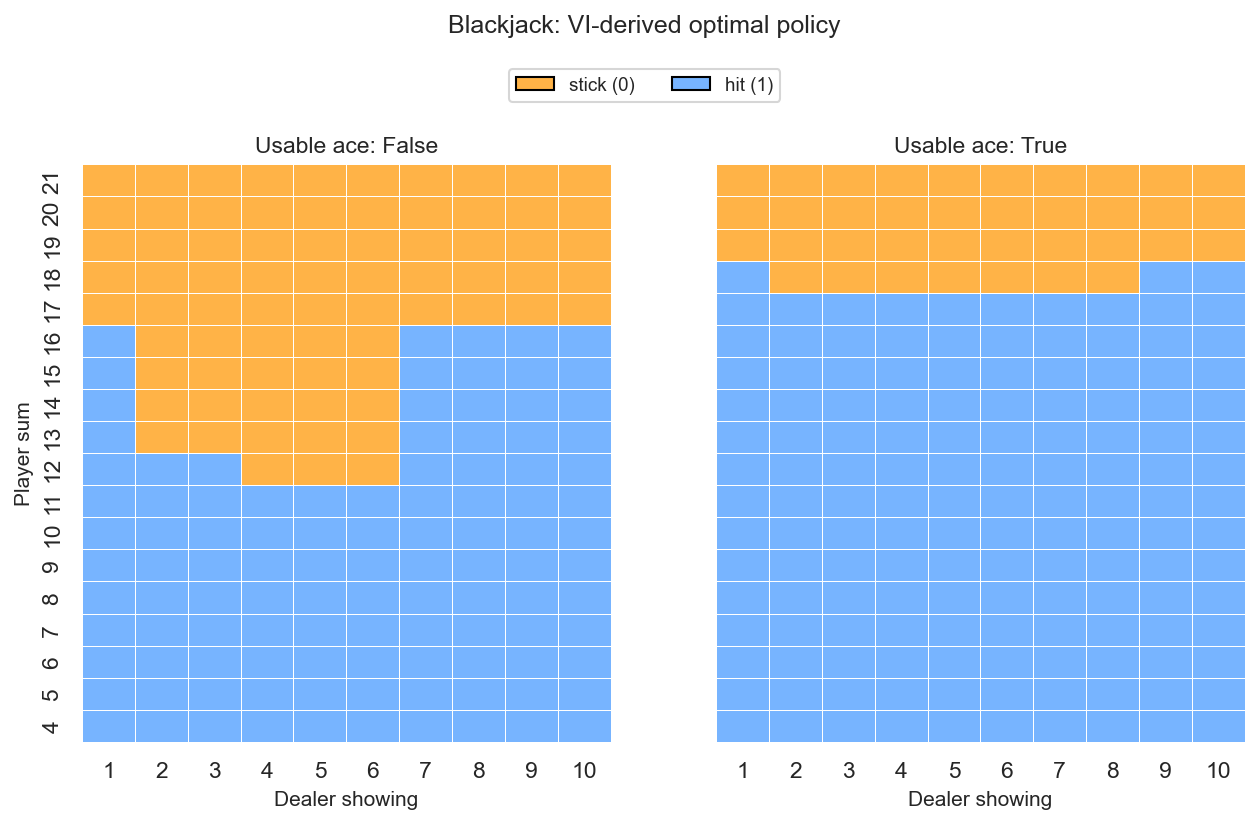
\includegraphics[width=\columnwidth]{figures/02_bj_policy_heatmap.png}
\caption{VI- and PI-derived Blackjack policies, projected onto player-sum /
dealer-card grids for the usable-ace and no-usable-ace cases. Panels agree
cell-for-cell, confirming $V^*_{\text{VI}} \equiv V^*_{\text{PI}}$.}
\label{fig:bj_policy_heatmap}
\end{figure}

\begin{figure*}[t]
\centering
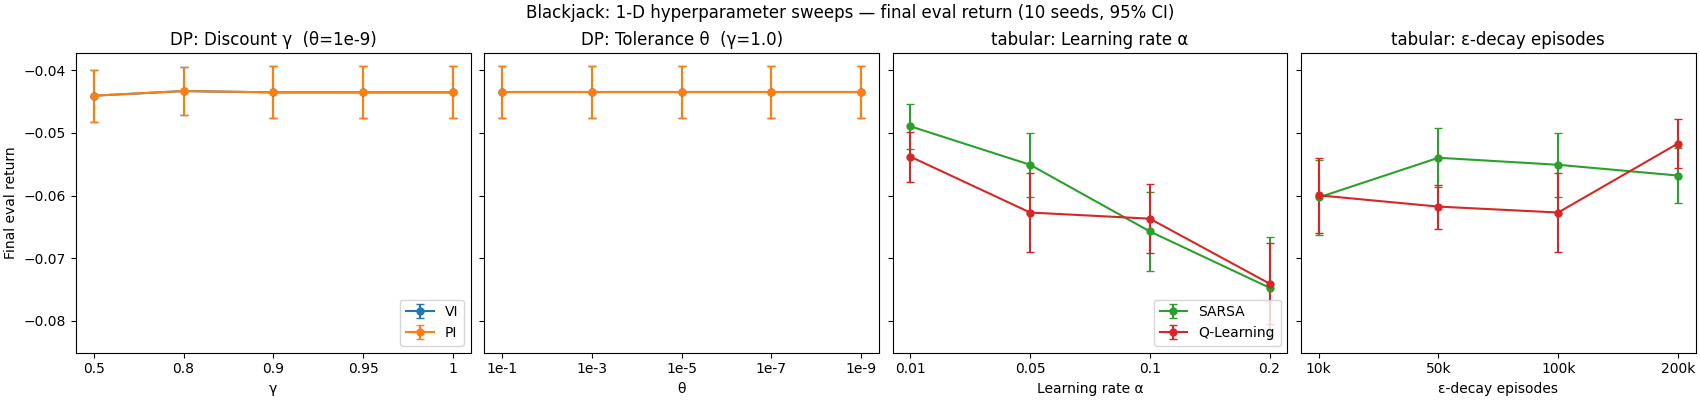
\includegraphics[width=\textwidth]{figures/04_bj_hp_sensitivity.png}
\caption{Blackjack 1-D hyperparameter sweeps --- final eval return
(10 seeds, 95\% CI). DP panels (left two) show VI and PI on the
analytical MDP; tabular panels (right two) show SARSA and
Q-Learning.}
\label{fig:bj_hp_sensitivity}
\end{figure*}

\begin{figure*}[t]
\centering
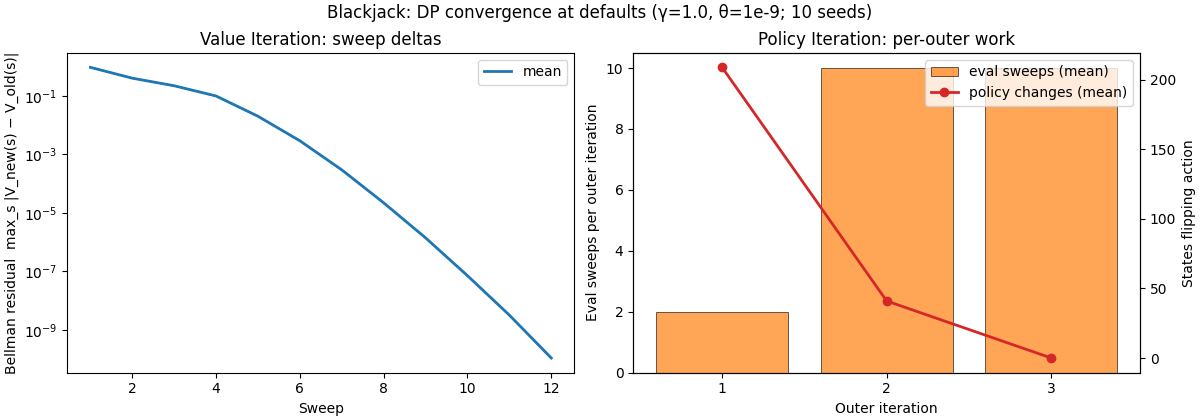
\includegraphics[width=0.72\textwidth]{figures/01_bj_dp_convergence.png}
\caption{Blackjack DP convergence at defaults
($\gamma = 1.0$, $\theta = 10^{-9}$). \emph{Left:} VI Bellman residual
per sweep, log scale. \emph{Right:} PI per-outer-iteration work ---
bars are PE sweeps, line is states flipping action.}
\label{fig:bj_dp_convergence}
\end{figure*}

\paragraph*{Solution quality.}
Figure~\ref{fig:bj_policy_heatmap} shows the VI- and PI-derived
policies overlapping cell-for-cell on both the usable-ace and
no-usable-ace grids, and the match holds on every seed. Default
eval return at $(\gamma = 1.0, \theta = 10^{-9})$ is
$-0.0435 \pm 0.004$ for both algorithms (20{,}000 eval episodes
per seed, 10 seeds). The left two panels of
Fig.~\ref{fig:bj_hp_sensitivity} extend this picture: eval return is
essentially flat at $-0.043$ to $-0.044$ across the full $\gamma$
sweep ($\gamma \in \{0.5, 0.8, 0.9, 0.95, 1.0\}$) and across the
full $\theta$ sweep ($10^{-1}$ to $10^{-9}$). Eval-return
$\gamma$-invariance is expected here: Blackjack rewards fire
only on terminal transitions, so every $\gamma$ scales the same
$\pm 1$ terminal reward uniformly across states and leaves the
greedy argmax --- and thus the policy and its eval return ---
unchanged. For DP on Blackjack, neither knob meaningfully moves
what the algorithm computes; both change only how much work it
takes to get there.

\paragraph*{Convergence cost.}
We measure cost in \emph{Bellman backups}: one evaluation of
$\sum_{s'} P(s'|s,a)[R + \gamma V(s')]$ for a single $(s,a)$. A
VI sweep costs $|\mathcal{S}|\cdot|\mathcal{A}|$ backups (all
actions for the $\max_a$); a PE sweep costs $|\mathcal{S}|$ (one
per state under the fixed policy); and each PI improvement step
adds another $|\mathcal{S}|\cdot|\mathcal{A}|$. For Blackjack
($|\mathcal{A}| = 2$), normalizing per state:
\[
  \text{VI bk}/|\mathcal{S}| = 2 N_{\text{VI}},
  \qquad
  \text{PI bk}/|\mathcal{S}| = N_{\text{PE}} + 2K,
\]
where $N_{\text{VI}}, N_{\text{PE}}$ are VI and total PE sweep
counts and $K$ is PI's outer-iteration count. Raw $K$ is
uninformative --- each outer round hides a full PE sub-loop ---
and wall-clock is noise-dominated ($\sim 1$\,s per configuration,
with $20$k-episode eval dwarfing the ms-scale DP solve). Bellman
backups are the only signal that moves with the convergence knobs.

At defaults ($\gamma = 1, \theta = 10^{-9}$;
Fig.~\ref{fig:bj_dp_convergence}), VI takes $12$ sweeps
($24$ bk/state); PI takes $K = 3$ outer iterations (zero seed
variance) with PE counts $(2, 10, 10) = 22$, giving $28$ bk/state
--- $\approx 1.17\times$ VI. Table~\ref{tab:bj_backups} sweeps
both knobs.

\begin{table}[!htbp]
\centering
\small
\caption{Blackjack DP convergence cost. Raw instrumentation
(VI sweeps $N_{\text{VI}}$, PI outer iterations $K$, PI total PE
sweeps $N_{\text{PE}}$) and derived per-state Bellman-backup
counts ($2 N_{\text{VI}}$ for VI; $N_{\text{PE}} + 2K$ for PI,
since $|\mathcal{A}| = 2$). Upper block: $\gamma$ sweep at
$\theta = 10^{-9}$. Lower block: $\theta$ sweep at $\gamma = 1.0$.}
\label{tab:bj_backups}
\begin{tabular}{@{}lrrrrrr@{}}
\toprule
 & $N_{\text{VI}}$ & $K$ & $N_{\text{PE}}$ &
 VI bk$/|\mathcal{S}|$ & PI bk$/|\mathcal{S}|$ & PI/VI \\
\midrule
\multicolumn{7}{@{}l}{\emph{$\gamma$ sweep ($\theta = 10^{-9}$)}} \\
$\gamma = 0.5$  & $10$ & $2$ & $11$ & $20$ & $15$ & $0.75$ \\
$\gamma = 0.9$  & $11$ & $2$ & $13$ & $22$ & $17$ & $0.77$ \\
$\gamma = 0.95$ & $12$ & $3$ & $23$ & $24$ & $29$ & $1.21$ \\
$\gamma = 1.0$  & $12$ & $3$ & $22$ & $24$ & $28$ & $1.17$ \\
\midrule
\multicolumn{7}{@{}l}{\emph{$\theta$ sweep ($\gamma = 1.0$)}} \\
$\theta = 10^{-1}$ & $4$  & $3$ & $8$  & $8$  & $14$ & $1.75$ \\
$\theta = 10^{-3}$ & $7$  & $3$ & $13$ & $14$ & $19$ & $1.36$ \\
$\theta = 10^{-5}$ & $9$  & $3$ & $17$ & $18$ & $23$ & $1.28$ \\
$\theta = 10^{-7}$ & $10$ & $3$ & $20$ & $20$ & $26$ & $1.30$ \\
$\theta = 10^{-9}$ & $12$ & $3$ & $22$ & $24$ & $28$ & $1.17$ \\
\bottomrule
\end{tabular}
\end{table}

\emph{Interpretation.} Both algorithms agree on policy and eval
return because they are Bellman operators on the same exact
$(T, R)$, and a finite proper MDP has a unique $V^*$. At the
backup level
(Table~\ref{tab:bj_backups}, PI/VI column), which algorithm wins
depends on $\gamma$, and the driver is $K$: it jumps from $2$ at
$\gamma \leq 0.9$ to $3$ at $\gamma \geq 0.95$. At $K = 2$, PI
is \emph{cheaper} than VI
(ratios $0.75$--$0.77$): PE's one-backup-per-state sweeps offset
the two extra improvement backups per outer round. At $K = 3$, the
extra PE round plus third improvement step tips the balance the
other way --- PI is $17$--$21\%$ more expensive than VI at $\theta = 10^{-9}$. PE itself saturates
at $\approx 10$ sweeps regardless of $\gamma$ because Blackjack is
a proper MDP with short expected horizon; the textbook ``PE
explodes as $\gamma \to 1$'' pathology applies to continuing tasks,
not episodic ones where every trajectory terminates with
probability $1$ and $V$ is bounded. The $\theta$ sweep at $\gamma = 1$ holds $K = 3$ fixed,
so PI/VI shrinks from $1.75$ at $\theta = 10^{-1}$ toward
$1.17$ at $\theta = 10^{-9}$ as PI's fixed improvement overhead
is amortized against growing PE counts.

\subsubsection{Tabular SARSA and Q-Learning}

\begin{figure}[t]
\centering
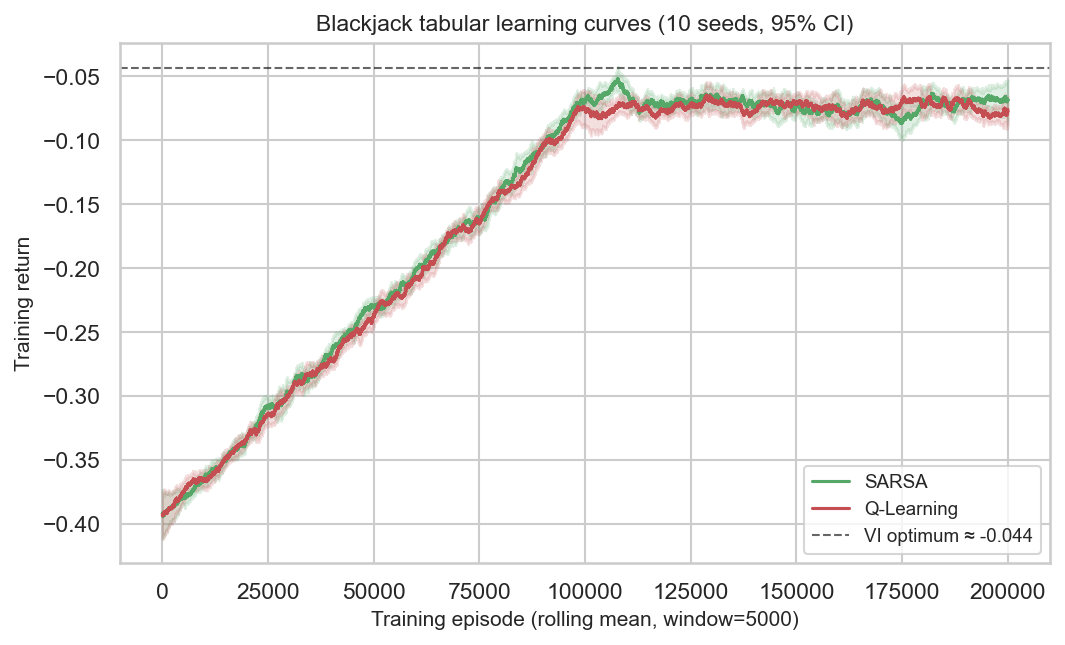
\includegraphics[width=\columnwidth]{figures/03_bj_tabular_curves.png}
\caption{Blackjack SARSA and Q-Learning training curves (mean over 10
seeds, shaded 95\% CI). Dashed line marks the VI-optimal eval return.}
\label{fig:bj_tabular_curves}
\end{figure}

At default hyperparameters (Table~\ref{tab:defaults}), SARSA
plateaus at $-0.0551 \pm 0.005$ and Q-Learning at
$-0.0627 \pm 0.006$, trailing the VI/PI Bellman-exact $-0.0435$
by $\sim$$0.012$ and $\sim$$0.019$ return respectively. Training
curves (Fig.~\ref{fig:bj_tabular_curves}) track closely throughout
and asymptote just below the VI-optimal dashed line.

The right two panels of Fig.~\ref{fig:bj_hp_sensitivity} show the
$\alpha$ and $\varepsilon$-decay sensitivity. Both algorithms peak at
$\alpha = 0.01$ (SARSA $-0.049$, Q-L $-0.054$), degrade monotonically
as $\alpha$ grows, and reach $\sim$$-0.075$ at $\alpha = 0.2$. The
$\varepsilon$-decay sweep shows Q-Learning preferring the slowest
schedule (200{,}000-episode decay, $-0.052$); SARSA is largely flat
across the range.

\emph{Interpretation.} SARSA and Q-Learning are statistically
close on Blackjack ($\Delta = 0.008$ return, within $\sim$$1$--$2$
CI half-widths) because the environment lacks the
``cliff-walking'' geometry that separates on- and off-policy
targets: SARSA's on-policy bootstrap and Q-Learning's off-policy
max only diverge when $\varepsilon$-exploration near a high-value
trajectory can tumble into a high-cost region. Blackjack has no
such structure --- every state is a few steps from a $\pm 1$
terminal reward --- so the two targets converge to essentially
the same values. At default $\alpha$, both algorithms plateau
$\sim$$0.012$ (SARSA) and $\sim$$0.019$ (Q-L) return below the
VI/PI Bellman-exact $-0.0435$; tuning $\alpha$ down to $0.01$
closes those gaps to $\sim$$0.005$ and $\sim$$0.010$. Both
algorithms prefer low $\alpha$ because Blackjack's sparse terminal
rewards make single-episode targets high-variance --- high
$\alpha$ overweights those noisy targets, low $\alpha$ averages
them. The residual $\sim$$0.005$--$0.010$ gap is a finite-sample
floor, not a structural one: tuned model-free \emph{approaches} DP on a
clean exact MDP but does not close the gap at $200{,}000$ training
episodes --- a concrete qualifier on H0. Q-Learning's preference for
the slowest $\varepsilon$-decay schedule is consistent with the
FAQ's warning that too-fast decay locks in premature exploitation
of an underexplored $Q$.

\begin{figure}[t]
\centering
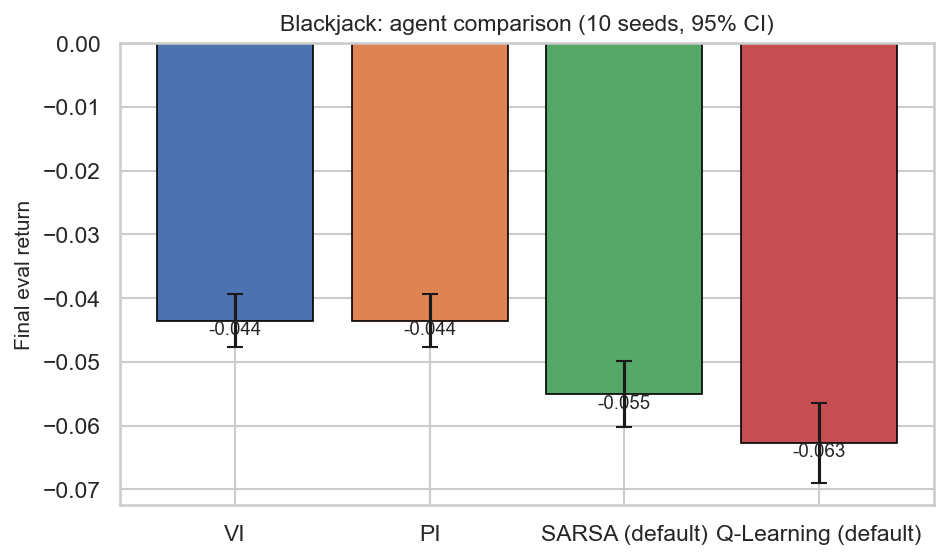
\includegraphics[width=\columnwidth]{figures/05_bj_agent_comparison.png}
\caption{Blackjack final eval return across VI, PI, SARSA (best
$\alpha$), and Q-Learning (best $\alpha$). VI $\equiv$ PI at the
Bellman-exact $-0.0435$; tuned SARSA trails by $\sim$$0.005$ and
tuned Q-Learning by $\sim$$0.010$ return.}
\label{fig:bj_agent_comparison}
\end{figure}

\subsection{CartPole}

\subsubsection{VI and PI on the estimated MDP}

\begin{figure}[t]
\centering
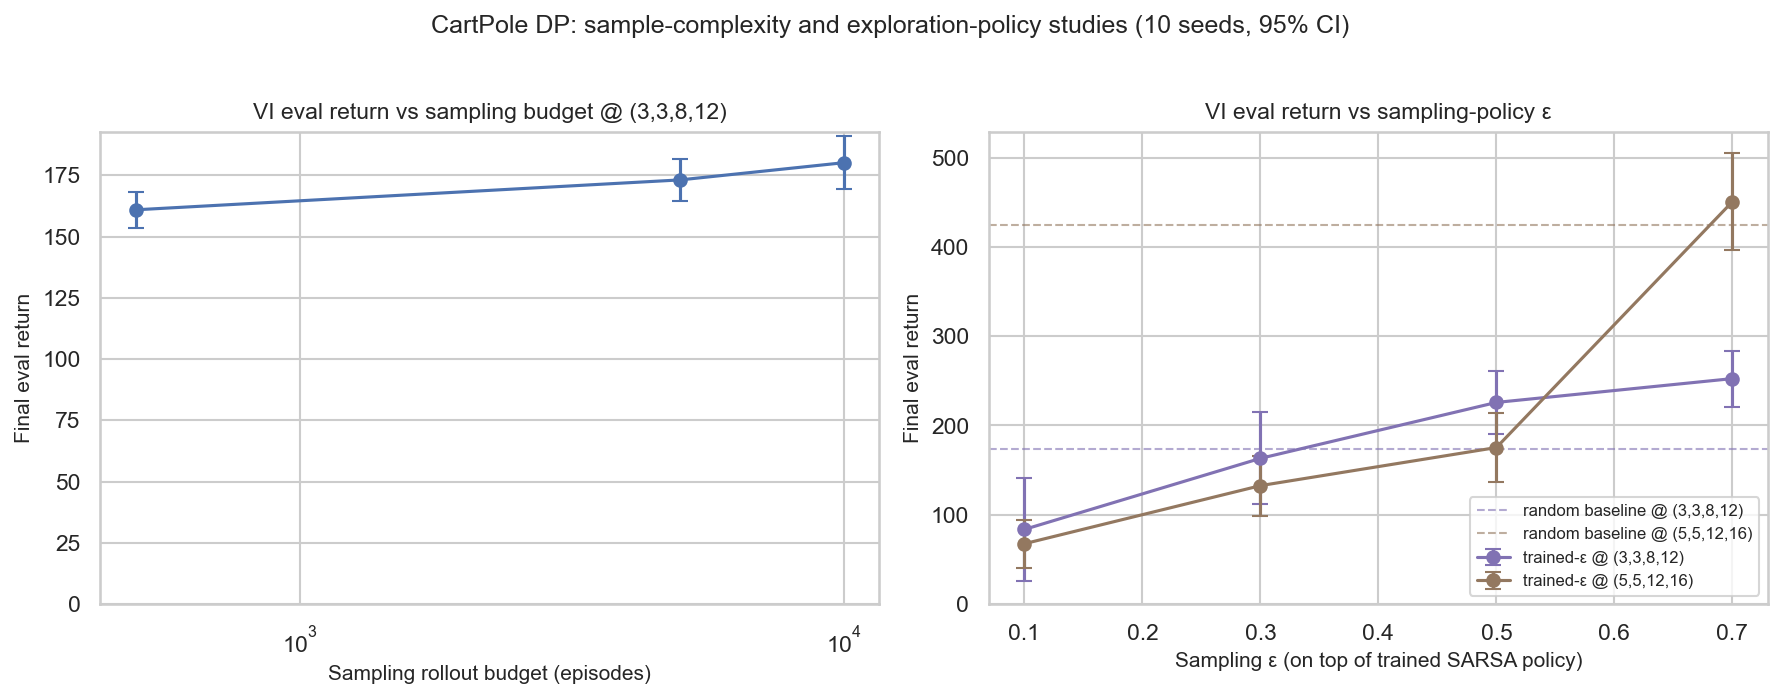
\includegraphics[width=\columnwidth]{figures/09_cp_dp_budget_and_eps.png}
\caption{DP on the estimated CartPole MDP. \emph{Left:} sample-budget
sweep at grid $(3, 3, 8, 12)$ with random sampling. \emph{Right:}
trained-SARSA $+\varepsilon$-greedy sampling across
$\varepsilon \in \{0.1, 0.3, 0.5, 0.7\}$ at two grids.}
\label{fig:cp_dp_budget_and_eps}
\end{figure}

\begin{figure}[t]
\centering
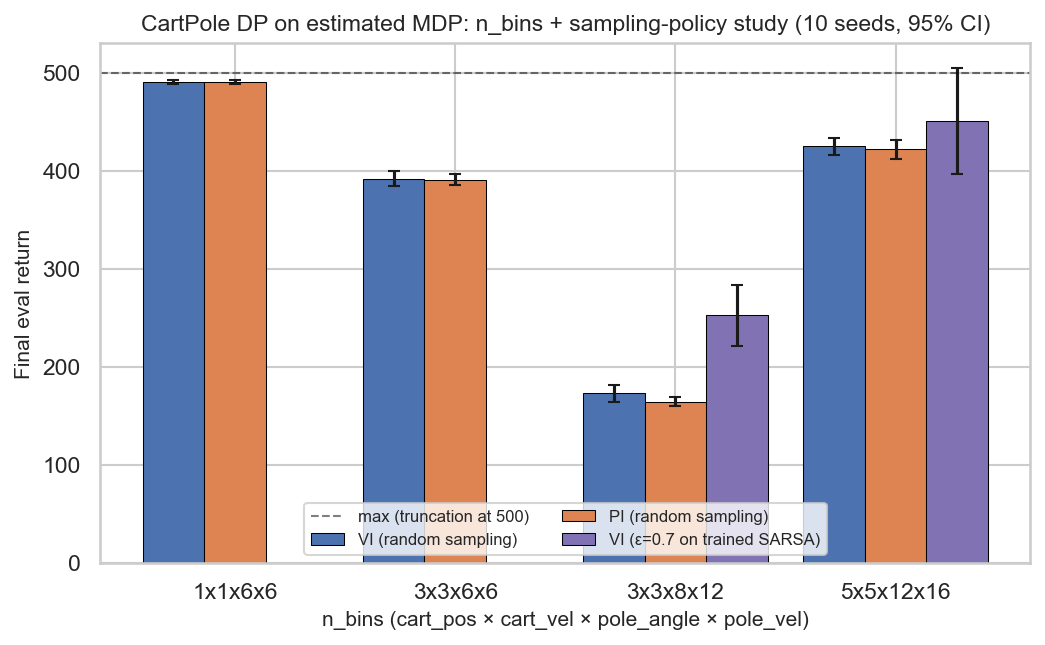
\includegraphics[width=\columnwidth]{figures/08_cp_dp_nbins.png}
\caption{VI/PI eval return on the estimated CartPole MDP across
four grids (random sampling); trained-SARSA $+\varepsilon$-greedy
sampling at $\varepsilon = 0.7$ overlaid at $(3,3,8,12)$ and
$(5,5,12,16)$. VI and PI overlap at every grid.}
\label{fig:cp_dp_nbins}
\end{figure}

\begin{table}[t]
\centering
\small
\setlength{\tabcolsep}{5pt}
\begin{tabular}{lccccc}
\toprule
 & Random & \multicolumn{4}{c}{Trained SARSA $+\varepsilon$-greedy} \\
\cmidrule(lr){2-2} \cmidrule(lr){3-6}
Grid & (baseline) & $\varepsilon = 0.1$ & $0.3$ & $0.5$ & $0.7$ \\
\midrule
$(3,3,8,12)$  & 173 & 84 & 163 & 226 & \textbf{253} \\
$(5,5,12,16)$ & 425 & 68 & 133 & 175 & \textbf{451} \\
\bottomrule
\end{tabular}
\caption{CartPole DP VI eval return at fixed $5{,}000$-rollout
budget, by sampling policy and grid. Bold = best per grid.}
\label{tab:cp_dp_eps_sweep}
\end{table}

Figures~\ref{fig:cp_dp_budget_and_eps}--\ref{fig:cp_dp_nbins} span
three sweeps; VI and PI agree within CI at every grid (default:
VI $173.1 \pm 8.6$ vs.\ PI $164.5 \pm 4.6$), so we report VI only.
A $20\times$ increase in random-rollout budget ($500 \to 10$k)
lifts VI eval return only $160.9 \to 180.2$ ($+12\%$). The grid
sweep under random sampling is non-monotonic in resolution:
$(1,1,6,6) \to \mathbf{490}$, $(3,3,6,6) \to 392$,
$(3,3,8,12) \to 173$, $(5,5,12,16) \to 425$. Sampling policy is
the dominant lever (Table~\ref{tab:cp_dp_eps_sweep}): at
$\varepsilon = 0.7$, trained-SARSA sampling lifts VI by $+79 / +26$
over random at the two grids, while low-$\varepsilon$ trained
sampling \emph{collapses} it to $84 / 68$. We did not
re-run trained-$\varepsilon$ sampling on the coarse grids: at
$(1,1,6,6)$ random is already within $10$ of the $500$-step
truncation ceiling (nowhere to go), and at $(3,3,6,6)$ the
$324$-cell space is small enough that random rollouts saturate
coverage --- trained sampling should give diminishing returns
exactly where the problem it targets (undersampled $(s, a)$ cells)
is not what's limiting performance.

\emph{Interpretation.} With an \emph{estimated} MDP, the Blackjack
story inverts. Algorithmic choice (VI vs.\ PI) becomes a noise
term --- CIs overlap at every grid --- but the
\emph{common} VI/PI eval return ranges from $\sim$$68$ (fine grid,
low-$\varepsilon$ trained sampling) to $\sim$$490$ (coarsest grid,
random), a $>$$7\times$ spread driven entirely by how the MDP is
\emph{estimated}. The budget sweep alone buys only $+12\%$, while
trained-$\varepsilon$ sampling at $\varepsilon = 0.7$ buys
$+26$--$79$ return points at fixed budget --- the $5{,}000$-rollout
baseline is not sample-starved, it is \emph{coverage-starved}. The
catastrophic failure at low $\varepsilon$ (Fig.~\ref{fig:cp_dp_budget_and_eps})
names the mechanism: a competent policy funnels rollouts into a
narrow tube of states it understands, leaving the rest of
$(s, a)$ space unvisited so the estimated $T$ treats it as
absorbing zero-reward sinks. The sweet spot at $\varepsilon = 0.7$
($\sim$30\% trained, 70\% random) anchors coverage on the
competent region while preserving breadth --- a sharper version
of our sampling-policy hypothesis (H2): trained $>$ random only
when perturbed heavily enough to preserve breadth.

The grid-sweep non-monotonicity (490 $\to$ 392 $\to$ 173 $\to$ 425)
falls out of the same coverage story. State count grows
combinatorially ($36 \to 324 \to 864 \to 4{,}800$ cells) while the
budget is held at $5{,}000$ rollouts; per-$(s, a)$ visit counts
drop by roughly an order of magnitude between the default and
finest grids. The dip at $(3,3,8,12)$ is a mid-range pathology:
fine enough to introduce cell distinctions that need filling,
coarse enough to still alias balance dynamics at the resolutions
that do get populated. The rebound at $(5,5,12,16)$ suggests that
once angle and angular-velocity resolution gets sharp enough to
capture the balance region cleanly, the remaining undersampled
cells become harmless --- random rollouts rarely reach them, and
the greedy policy stays inside the well-covered core.

The $(1,1,6,6)$ result deserves a separate callout. DP scores
$\mathbf{490.5 \pm 1.6}$, nearly saturating the 500-step truncation
ceiling, on a grid that collapses the entire cart axis ($x,
\dot{x}$) into a single bin. This works because CartPole's
balance dynamics are approximately decoupled from cart position:
the pole falls due to angle and angular velocity, not where the
cart is on the track. A 1-bin cart axis is therefore equivalent
to ``ignore cart position entirely,'' which is viable. This result
stands as the cleanest single illustration of H0 in the campaign
(see H0 Resolution, \S\ref{sec:hyp_resolution}).

\subsubsection{Tabular SARSA and Q-Learning}

\begin{figure}[t]
\centering
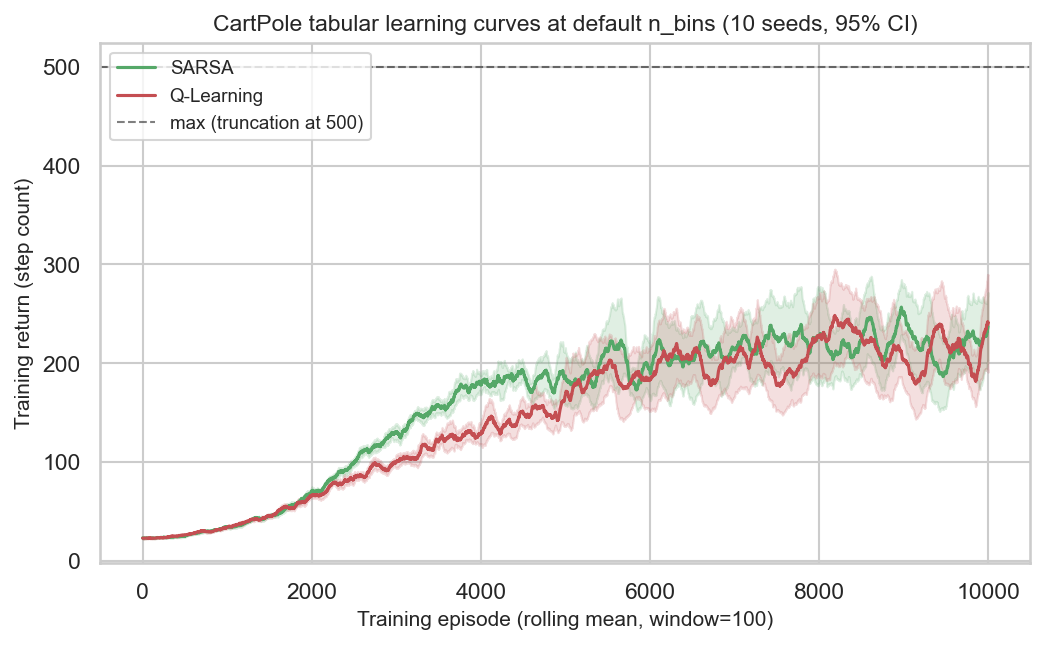
\includegraphics[width=\columnwidth]{figures/06_cp_tabular_curves.png}
\caption{CartPole (default grid) SARSA and Q-Learning training curves.}
\label{fig:cp_tabular_curves}
\end{figure}

\begin{table}[t]
\centering
\small
\setlength{\tabcolsep}{4pt}
\begin{tabular}{lcccc}
\toprule
 & \multicolumn{4}{c}{Learning rate $\alpha$} \\
\cmidrule(lr){2-5}
 & 0.05 & 0.1 & 0.2 & 0.5 \\
\midrule
SARSA & 226 & \textbf{298} & 206 & 223 \\
Q-L   & 225 & 267 & \textbf{292} & 171 \\
\midrule
 & \multicolumn{4}{c}{Discount $\gamma$} \\
\cmidrule(lr){2-5}
 & 0.9 & 0.95 & 0.99 & 1.0 \\
\midrule
SARSA & 221 & 252 & \textbf{298} & 224 \\
Q-L   & 232 & 179 & \textbf{267} & 248 \\
\midrule
 & \multicolumn{4}{c}{Grid $(x, \dot x, \theta, \dot\theta)$} \\
\cmidrule(lr){2-5}
 & (1,1,6,6) & (3,3,6,6) & (3,3,8,12) & (5,5,12,16) \\
\midrule
SARSA & 224 & 288 & \textbf{298} & 206 \\
Q-L   & 168 & 266 & \textbf{267} & 224 \\
\bottomrule
\end{tabular}
\caption{CartPole tabular HP sweeps, final eval return (10 seeds).
Bold marks each row's peak. Defaults: $\alpha = 0.1$,
$\gamma = 0.99$, grid $(3,3,8,12)$.}
\label{tab:cp_tabular_sweeps}
\end{table}

Table~\ref{tab:cp_tabular_sweeps} summarizes three HP sweeps around
default eval returns SARSA $297.99 \pm 71.15$ and Q-Learning
$267.39 \pm 81.37$ (Fig.~\ref{fig:cp_tabular_curves}). All three
sweeps peak near the defaults and degrade in both directions;
the one anomaly is Q-L's $\gamma = 0.95 \to 179$ dip.

\emph{Interpretation.} SARSA $\approx$ Q-Learning throughout
($\Delta = 31$ return at default HPs, well within a CI half-width;
the two curves stay inside each other's CIs across every sweep
point): CartPole's uniform ``$+1$ per surviving step'' reward has
no cliff-walking structure either, so the on- and off-policy
targets converge to essentially the same $Q$ (H3). The interesting
structure is on the other axes.

The grid sweep peaks at the default $(3,3,8,12)$ for both
algorithms and drops off in both directions
(Table~\ref{tab:cp_tabular_sweeps}). Adding
cart-position bins at the coarsest pole resolution
($(1,1,6,6) \to (3,3,6,6)$) lifts SARSA by $+64$ and Q-Learning
by $+98$; further refining the pole axis
($(3,3,6,6) \to (3,3,8,12)$) adds only $+10 / +1$; and the finest grid
$(5,5,12,16)$ \emph{regresses} on both ($-92 / -43$), because the
10{,}000-episode sample budget is now spread across $4{,}800$
cells instead of $864$ --- tabular performance is bounded by
samples, not grid detail. This sample-starvation confound makes
it hard to cleanly isolate H4's angular-over-cart-position
sub-claim at the finest grid.

Both algorithms are $\gamma$-sensitive with a peak at $\gamma = 0.99$
and lower returns on either side --- Blackjack's
$\gamma$-invariance does not carry over to a long-horizon,
per-step-reward environment. The Q-Learning dip at
$\gamma = 0.95 \to 179$ is anomalous and likely seed variance at
the edge of the algorithm's stable region; $10$ seeds is small
enough that one or two outliers move the mean materially. Overall
H4 holds qualitatively --- CartPole is $\gamma$- and grid-sensitive
--- with sample-starvation and seed variance as honest qualifiers.

\subsubsection{DQN baseline and Rainbow-medium ablation (EC)}

\begin{figure}[t]
\centering
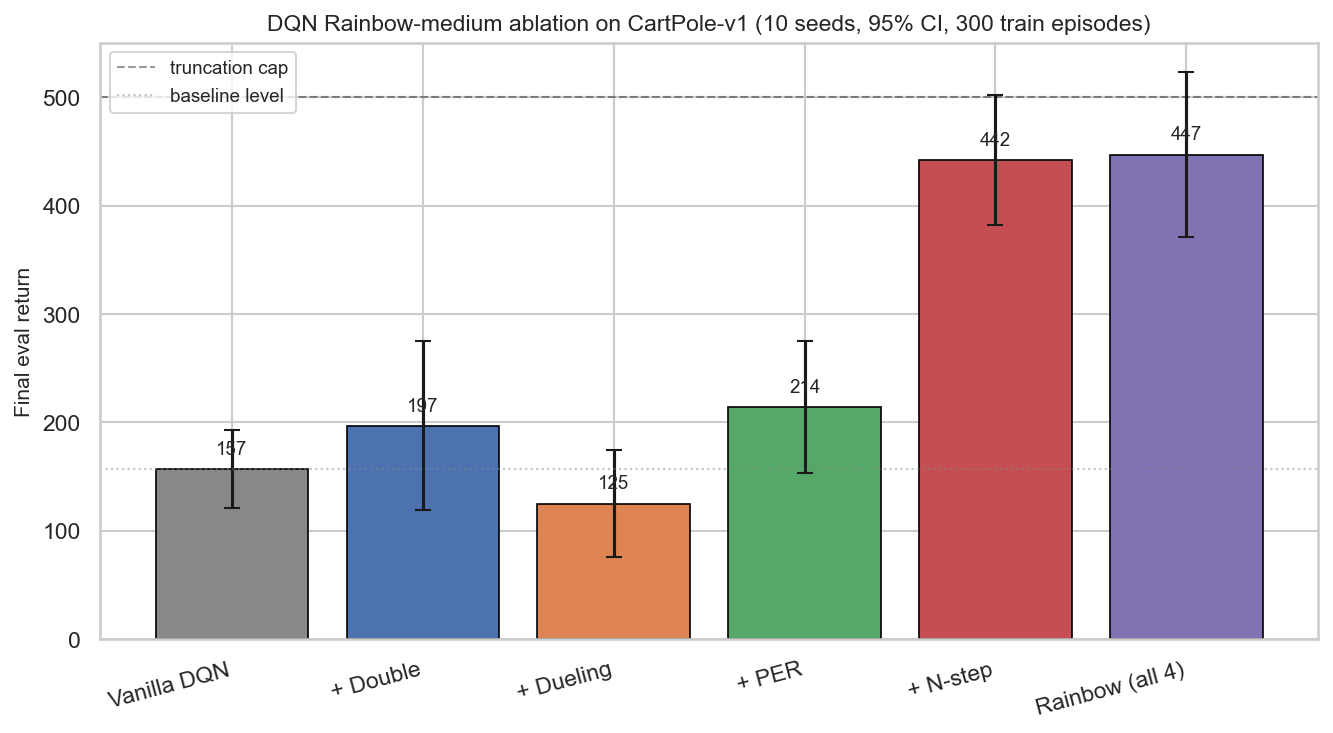
\includegraphics[width=\columnwidth]{figures/11_dqn_ablation_bars.png}
\caption{Rainbow-medium ablation final eval return (10 seeds, 95\% CI).
Components: \{baseline, double, dueling, per, n-step, rainbow\}.}
\label{fig:dqn_ablation_bars}
\end{figure}

\begin{figure}[t]
\centering
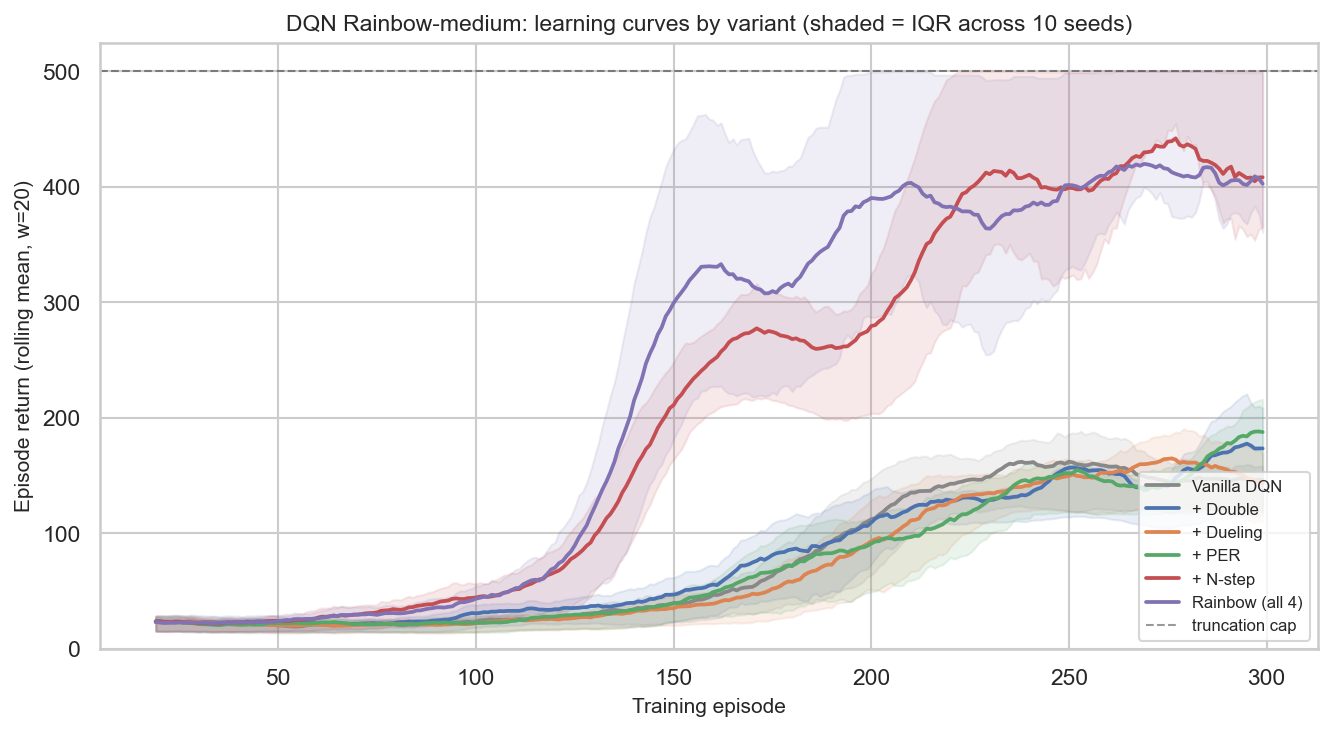
\includegraphics[width=\columnwidth]{figures/12_dqn_learning_curves.png}
\caption{DQN learning curves per variant. Rainbow combines all four
toggles.}
\label{fig:dqn_learning_curves}
\end{figure}

Final eval returns across the six variants (10 seeds, 95\% CI), each
trained for a matched 300-episode budget
(Fig.~\ref{fig:dqn_ablation_bars}):
\begin{itemize}
\itemsep0em
\item baseline DQN: $157.2 \pm 36.0$,
\item + Double~\cite{vanhasselt2016}: $196.8 \pm 77.9$~~($\Delta = +40$),
\item + Dueling~\cite{wang2016}: $125.1 \pm 49.6$~~($\Delta = -32$),
\item + PER~\cite{schaul2016}: $214.1 \pm 61.0$~~($\Delta = +57$),
\item + $n$-step~\cite{sutton1988}: $441.9 \pm 59.9$~~($\Delta = +285$),
\item Rainbow-medium (all four): $447.0 \pm 76.2$~~($\Delta = +290$).
\end{itemize}
Rainbow-full is indistinguishable from $n$-step alone within 95\% CI.
Learning curves (Fig.~\ref{fig:dqn_learning_curves}) show DQN-baseline
with pronounced episode-to-episode variance and periodic regressions;
Rainbow-medium curves are noticeably smoother.

\emph{Interpretation.} H5's first prediction --- vanilla DQN beats
tabular Q-Learning because function approximation matches a continuous
state space --- does \emph{not} hold at our 300-episode budget: DQN
baseline reaches $157$ against tabular's $267$--$298$. The
function-approximation machinery (replay buffer, target network, Huber
loss) buys long-run stability at the cost of a warm-up period: the
buffer needs to fill, the target net updates on a delay, and gradient
updates smooth over many transitions before a usable $Q$ emerges.
Tabular agents pay no such warm-up cost --- each $(s, a, r, s')$
updates a single cell immediately --- so at $300$ episodes tabular is
ahead.

The ablation story is sharper than we predicted. $n$-step alone
captures essentially all of Rainbow's gain ($+285$ vs.\
Rainbow-full's $+290$, within noise); PER adds $+57$; Double adds
$+40$; and Dueling \emph{actively regresses} ($-32$).

Why does $n$-step dominate? Early in training, CartPole episodes
last only $10$--$50$ steps before the pole falls, so the main
bottleneck is that reward signal propagates backward slowly through
1-step bootstrapping. $n$-step ($n = 3$) bootstraps from three
actual rewards instead of one, propagating signal $3\times$ faster
and directly cutting target variance. The other three components
target different problems: PER picks which transitions to replay
(helps sample efficiency, doesn't change the target itself); Double
uses a separate network to pick the max action in the target
(reduces overestimation bias, not variance); and Dueling splits the
output into state-value and advantage heads, which on a $2$-action
problem with a small MLP adds parameters and complexity without a
clean payoff, which we think likely explains the negative delta. That $n$-step alone
$\approx$ Rainbow-full means the four components do \emph{not}
compose at our scale; the Rainbow paper's ``each component adds
something'' claim~\cite{hessel2018} does not hold here. H0 still
prevails in the end: Rainbow-medium ($447$) clears the tabular
ceiling ($\sim 298$), but the representation benefit only
materializes once $n$-step is layered on.

\begin{figure}[t]
\centering
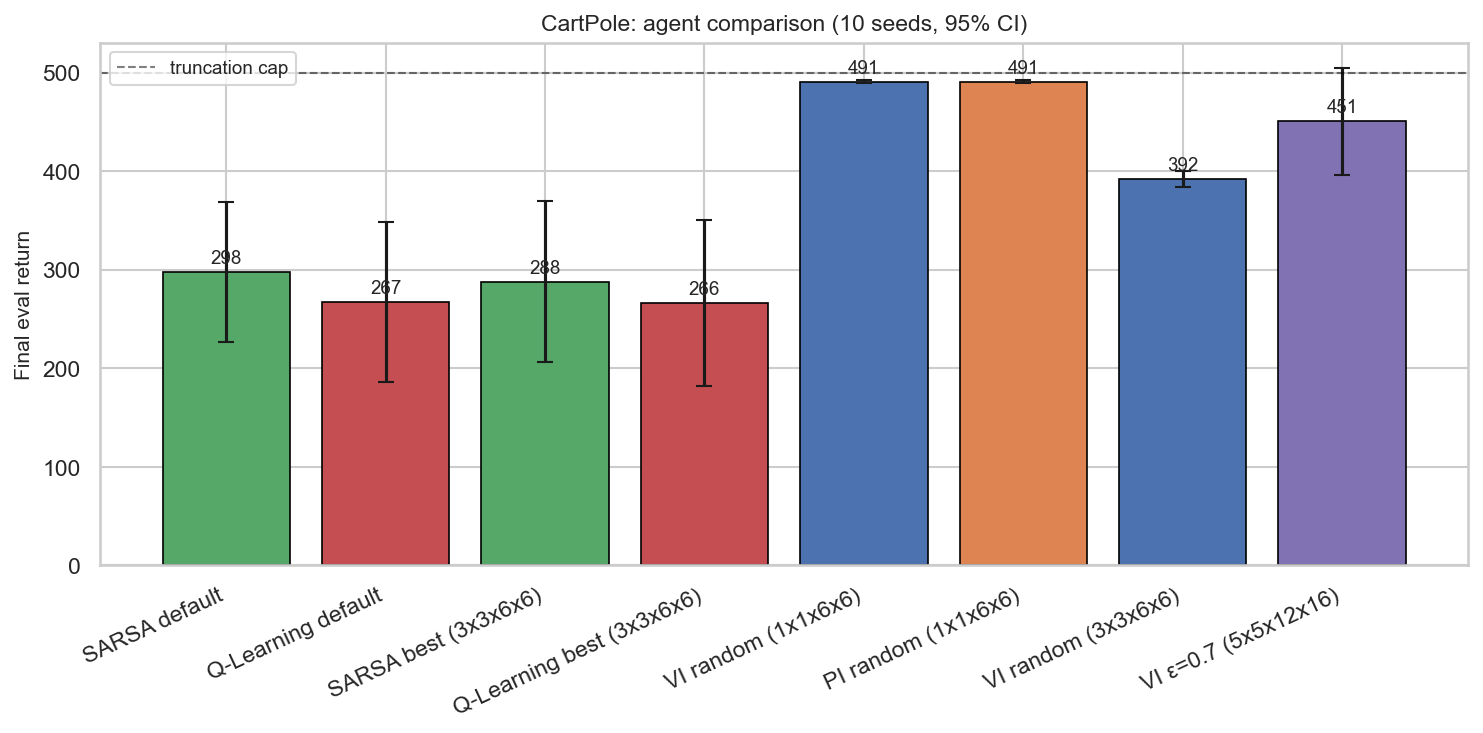
\includegraphics[width=\columnwidth]{figures/10_cp_agent_comparison.png}
\caption{CartPole final eval return across agent configurations,
including DP on the estimated MDP at multiple grids.}
\label{fig:cp_agent_comparison}
\end{figure}


%%%%%%%%%%%%%%%%%%%%%%%%%%%%%%%%%%%%%%%%%%%%%%%%%%%%%%%%%%%%%%%%%%%%%%%%%%%%%%%%
\section{Hypothesis Resolution}
\label{sec:hyp_resolution}

\textbf{H0 (meta).} Partially supported, with qualifier. Blackjack is
unambiguously DP's home turf: VI/PI find the exact optimum in 1\,s
wall-clock, while tabular model-free (best-tuned $\alpha$) plateaus
$0.005$--$0.010$ return short after 200{,}000 training episodes. On CartPole, DP wins at coarse grids
($490$ at $(1,1,6,6)$), but it can also fail spectacularly ($173$ at
$(3,3,8,12)$ under random sampling), and model-free wins at medium
grids. The ``pick the algorithm family that matches the MDP structure''
slogan is correct on average but hides a second axis: \emph{on
continuous MDPs, DP's success also depends on getting the
discretization and sampling policy right}. Model-free has fewer knobs
that can go this catastrophically wrong. The two families also fail
for different reasons: tabular model-free is bounded by samples
(degrades at the finest grid where $10{,}000$ episodes cannot cover
$4{,}800$ cells), whereas DP on the estimated MDP is bounded by
coverage (degrades when the sampling distribution funnels too
narrowly) --- the two bottlenecks bind at different grids, which
is why ``best family'' changes with discretization.

\textbf{H1 (Blackjack DP).} Partially supported. Policies match
to four significant figures at every $\gamma$, as predicted. The
backup prediction is only right at high $\gamma$: PI is $17$--$21\%$
\emph{more} expensive than VI for $\gamma \geq 0.95$, but $23$--$25\%$
\emph{cheaper} for $\gamma \leq 0.9$. The driver is $K$
(PI outer iterations: 2 at low $\gamma$, 3 at high), not the
contraction-rate story --- Blackjack's bounded horizon caps PE
at $\approx 10$ sweeps regardless of $\gamma$.

\textbf{H2 (CartPole DP sampling).} Supported, with sharper
framing. Trained-$\varepsilon$ at $\varepsilon = 0.7$ lifts VI by
$+79 / +26$ at the two grids. But at low $\varepsilon$
($0.1$--$0.3$), trained sampling \emph{loses} to random by
$10$--$357$ points (worst on the finer grid) --- coverage, not
competence, is binding.

\textbf{H3 (SARSA $\approx$ Q-L).} Supported. Blackjack
$\Delta = 0.008$ return; CartPole $\Delta = 31$ at default HPs
(within one CI half-width), and the two curves stay inside each
other's CIs across every $\alpha$, $\gamma$, and grid sweep
point. Neither environment shows the cliff-walking-style
bias-driven separation H3 flagged as the usual failure mode.

\textbf{H4 (discretization + $\gamma$).} Partially supported. The
$\gamma$ sub-claim holds cleanly: $\gamma = 0.99$ is CartPole's
clear optimum, and Blackjack $\gamma$-invariance is confirmed
across five values. The pole-dominates-cart sub-claim is
confounded by sample starvation --- cart-axis refinement actually
lifts performance more than pole-axis refinement in our sweep,
but the finest grid regresses, so we cannot cleanly isolate the
axis effect.

\textbf{H5 (DQN $>$ tabular, Rainbow composition).} Both
predictions refuted at our scale. DQN-baseline ($157$)
underperforms tabular Q-L ($267$) at 300 episodes. Within Rainbow,
$n$-step alone ($+285$) captures all of Rainbow-full's gain
($+290$); Dueling \emph{regresses} ($-32$). Rainbow does beat
tabular in the end ($447$ vs.\ ceiling $\sim 298$), validating
H0's representation-matching intuition, but only once $n$-step
is layered on.

\textbf{Synthesis.} Pulling back from the five verdicts, the
sharpest cross-cutting takeaway is the \emph{two failure modes}
story: tabular model-free and DP-on-estimated-MDP hit different
bottlenecks. Tabular is sample-bound --- $10{,}000$ episodes
cannot cover $4{,}800$ cells at the finest grid. DP on the
estimated MDP is coverage-bound --- fixed-budget rollouts leave
regions of $(s, a)$-space unvisited, which the estimated $T$ then
treats as absorbing zero-reward. The two bottlenecks show up at
different grid sizes, which is why the ``best family'' shifts
with discretization: a refinement of H0's static ``match
algorithm to MDP structure'' slogan that Blackjack alone would
not reveal. Two secondary insights stand out. First, Blackjack's
PI/VI comparison corrects a common textbook intuition: ``PE
explodes as $\gamma \to 1$'' applies to continuing tasks, not
proper episodic MDPs where bounded horizons cap PE at $\approx 10$
sweeps --- the real driver of PI's cost was $K$ (outer iterations:
$2$ at $\gamma \leq 0.9$, $3$ at $\gamma \geq 0.95$), not
contraction rate. Second, within Rainbow-medium, $n$-step returns
alone capture $98\%$ of the ablation's gain and Dueling actively
regresses on this small MLP; at 300-episode scale, the practical
recommendation is to reach for $n$-step first and Dueling last.


%%%%%%%%%%%%%%%%%%%%%%%%%%%%%%%%%%%%%%%%%%%%%%%%%%%%%%%%%%%%%%%%%%%%%%%%%%%%%%%%
\section{Limitations and Future Work}

The CartPole tabular-vs-DQN comparison fixes the tabular grid at
the default $(3, 3, 8, 12)$; a more thorough study would tune
$\alpha$ and $\varepsilon$-decay \emph{within} each grid, since
the optima likely depend on cell count. Our DQN EC runs at a
$300$-episode training budget to keep total compute tractable;
longer budgets would likely narrow the DQN-baseline gap to tabular
Q-Learning, though we expect Rainbow-medium to retain its
advantage. We also explicitly drop C51 and NoisyNets up front, so
our findings cover a four-of-six Rainbow-medium ablation rather
than the full Rainbow paper. Our Blackjack MDP is hand-written
against the Gymnasium \texttt{Blackjack-v1} rules; a useful future
validation would be to compare our transition probabilities
against empirical Gym rollouts. Finally, the trained-$\varepsilon$
sampling study uses \emph{SARSA}-pretrained policies as the
sampling source; we did not rerun it with Q-Learning-pretrained
policies. Given H3's finding that SARSA and Q-Learning are
indistinguishable on CartPole, we expect the result to carry over,
but we stop short of asserting it.


%%%%%%%%%%%%%%%%%%%%%%%%%%%%%%%%%%%%%%%%%%%%%%%%%%%%%%%%%%%%%%%%%%%%%%%%%%%%%%%%
\section*{AI Use Statement}
I used Cursor (Claude) to generate and refactor experiment code, produce
plots, and assist with report drafting and outlining. I thoroughly reviewed,
verified, and understand all AI-assisted content, and all final analysis and
conclusions are my own.


%%%%%%%%%%%%%%%%%%%%%%%%%%%%%%%%%%%%%%%%%%%%%%%%%%%%%%%%%%%%%%%%%%%%%%%%%%%%%%%%
\begin{thebibliography}{99}

\bibitem{sutton2018}
R.~S.~Sutton and A.~G.~Barto,
\emph{Reinforcement Learning: An Introduction}, 2nd ed.
Cambridge, MA, USA: MIT Press, 2018, Example 5.3 ``Blackjack.''

\bibitem{barto1983}
A.~G.~Barto, R.~S.~Sutton, and C.~W.~Anderson,
``Neuronlike adaptive elements that can solve difficult learning control
problems,''
\emph{IEEE Trans.\ Syst., Man, Cybern.}, vol.~SMC-13, no.~5,
pp.~834--846, Sep.--Oct.\ 1983, doi:10.1109/TSMC.1983.6313077.

\bibitem{gym_blackjack}
Farama Foundation,
``Blackjack-v1,'' \emph{Gymnasium Documentation}, 2023. [Online]. Available:
\url{https://gymnasium.farama.org/environments/toy_text/blackjack/}

\bibitem{gym_cartpole}
Farama Foundation,
``CartPole-v1,'' \emph{Gymnasium Documentation}, 2023. [Online]. Available:
\url{https://gymnasium.farama.org/environments/classic_control/cart_pole/}

\bibitem{cartpole_faq}
T.~LaGrow,
\emph{CS 7641 Reinforcement Learning Report FAQ, Spring 2026}.
Georgia Institute of Technology, Atlanta, GA, USA, 2026.

\bibitem{howard1960}
R.~A.~Howard,
\emph{Dynamic Programming and Markov Processes}.
Cambridge, MA, USA: MIT Press, 1960.

\bibitem{mnih2015}
V.~Mnih \emph{et al.},
``Human-level control through deep reinforcement learning,''
\emph{Nature}, vol.~518, no.~7540, pp.~529--533, Feb.\ 2015.

\bibitem{vanhasselt2016}
H.~van Hasselt, A.~Guez, and D.~Silver,
``Deep reinforcement learning with double Q-learning,''
in \emph{Proc.\ AAAI Conf.\ Artif.\ Intell.}, vol.~30, no.~1, 2016,
pp.~2094--2100.

\bibitem{wang2016}
Z.~Wang, T.~Schaul, M.~Hessel, H.~van Hasselt, M.~Lanctot, and N.~de Freitas,
``Dueling network architectures for deep reinforcement learning,''
in \emph{Proc.\ 33rd Int.\ Conf.\ Mach.\ Learn.}, New York, NY, USA,
2016, pp.~1995--2003.

\bibitem{schaul2016}
T.~Schaul, J.~Quan, I.~Antonoglou, and D.~Silver,
``Prioritized experience replay,''
in \emph{Proc.\ 4th Int.\ Conf.\ Learn.\ Represent.}, San Juan, Puerto
Rico, 2016.

\bibitem{sutton1988}
R.~S.~Sutton,
``Learning to predict by the methods of temporal differences,''
\emph{Mach.\ Learn.}, vol.~3, no.~1, pp.~9--44, Aug.\ 1988.

\bibitem{hessel2018}
M.~Hessel \emph{et al.},
``Rainbow: Combining improvements in deep reinforcement learning,''
in \emph{Proc.\ 32nd AAAI Conf.\ Artif.\ Intell.}, New Orleans, LA, USA,
2018, pp.~3215--3222.

\end{thebibliography}

\end{document}
